\StartAppendix
\chapter{การ Deploy แอปพลิเคชัน}
\section{การ Build แอปพลิเคชันเป็นไฟล์รูปแบบ .apk สำหรับสมาร์ตโฟนระบบปฏิบัติการ Android}
การ Build แอปพลิเคชันเป็นไฟล์รูปแบบ .apk ในการพัฒนาแอปพลิเคชันด้วย Flutter นั้นมีขั้นตอนดังนี้
\begin{enumerate}
    \item เปิดหน้าต่าง Flutter Project ที่พัฒนาขึ้น (ในที่นี้ผู้พัฒนาใช้โปรแกรม Microsoft Visual Studio Code ในการพัฒนา)
    \begin{figure}
        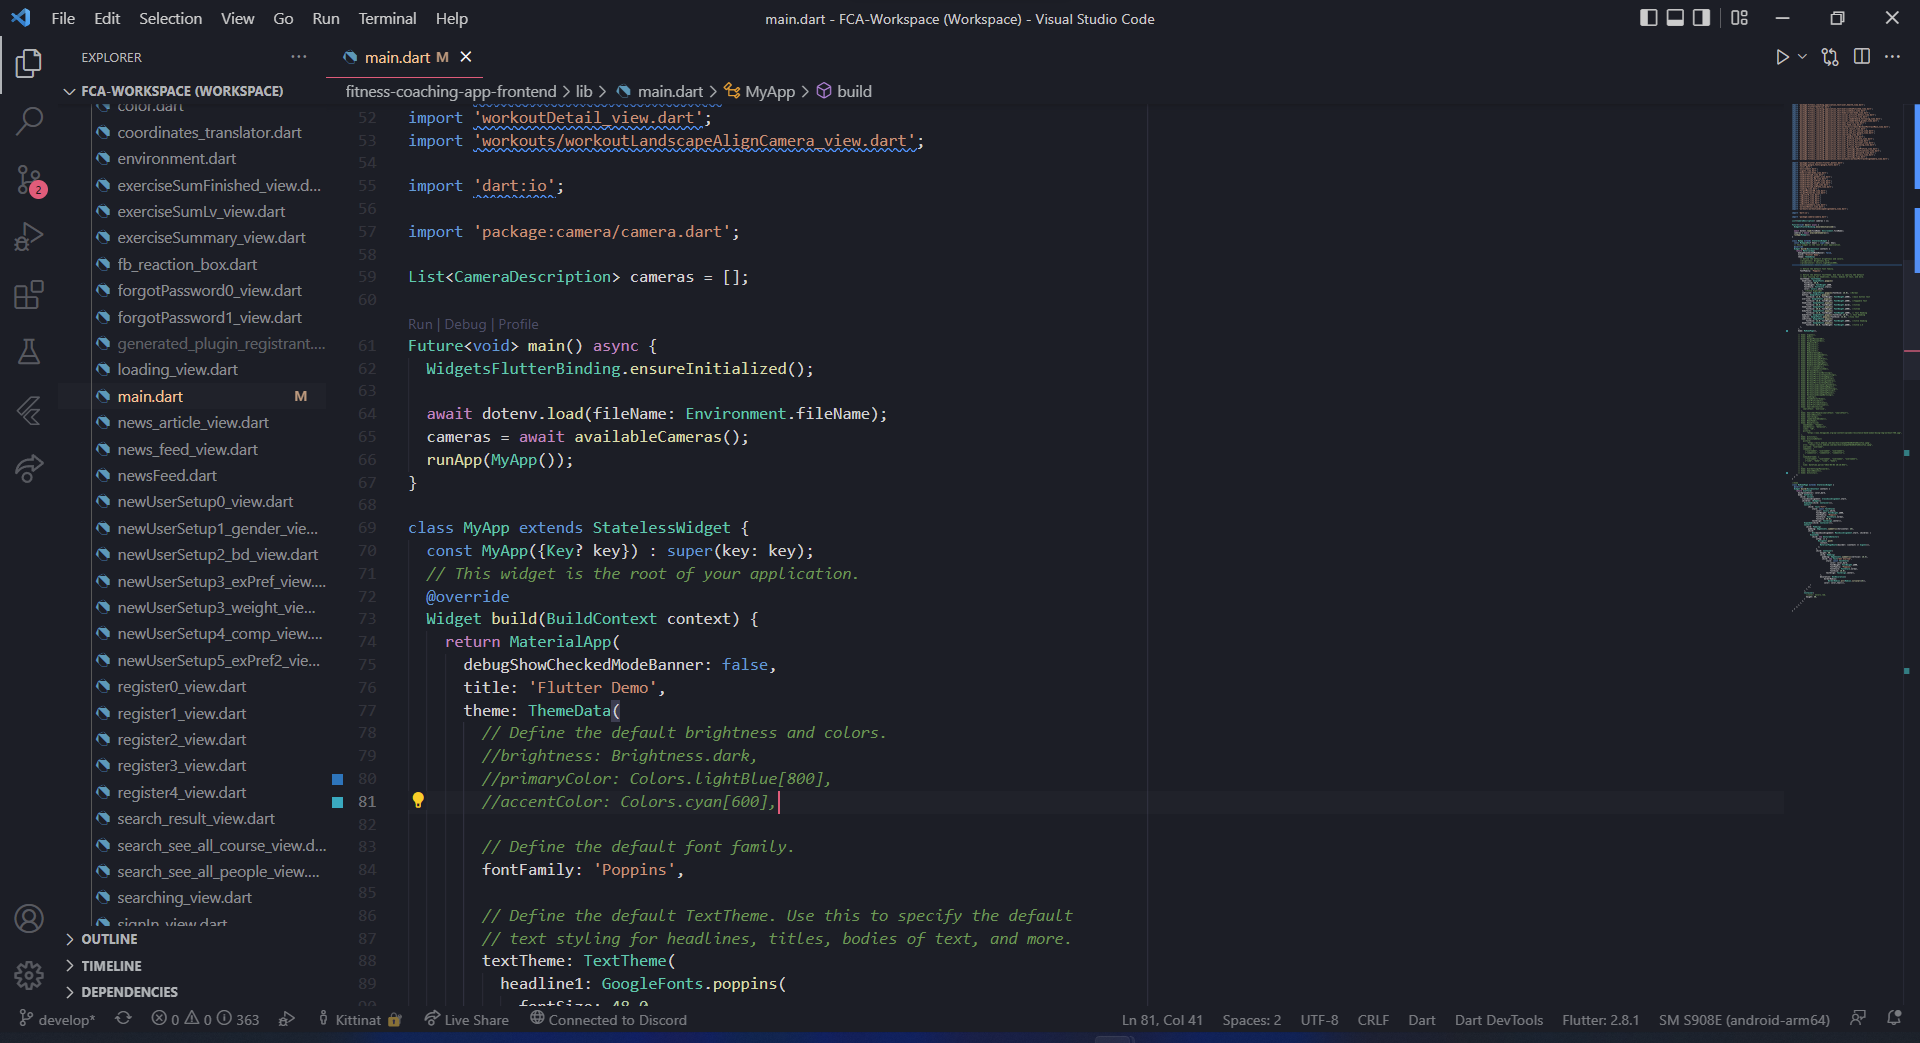
\includegraphics[width=15cm]{./appendix/a-1.png}
        \caption{หน้าต่าง Flutter Project ที่พัฒนา}
    \end{figure}
    \item เปิดหน้าต่าง Terminal โดยการคลิกที่ Terminal ในแถบ Menu Bar จากนั้นคลิกที่ New Terminal โปรแกรมจะทำการเปิดหน้าต่าง Terminal ขึ้นที่บริเวณส่วนล่างของจอ
    \begin{figure}
        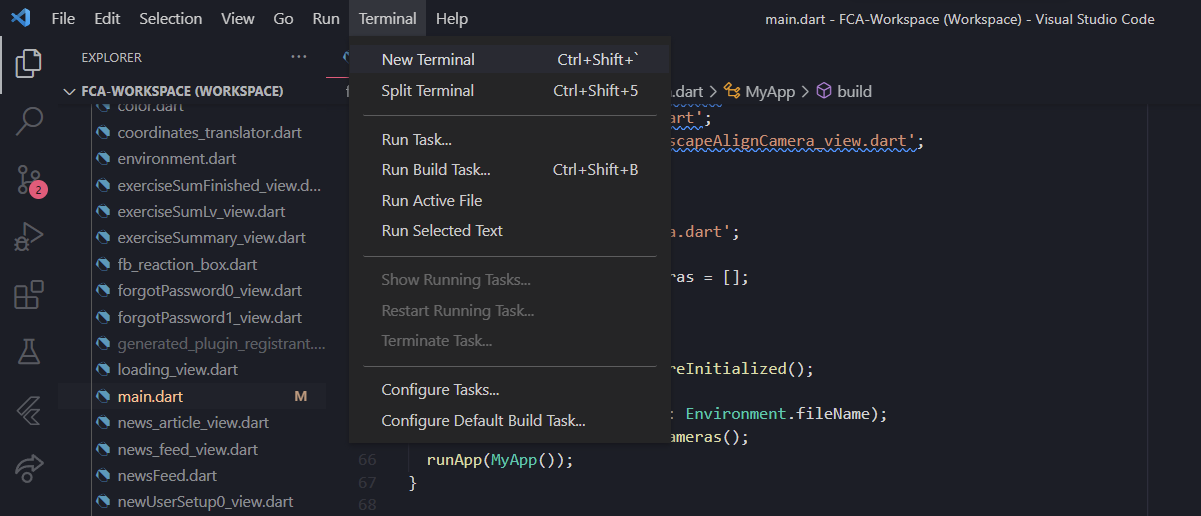
\includegraphics[width=15cm]{./appendix/a-2.png}
        \caption{การเปิดหน้าต่าง Terminal}
    \end{figure}
    \begin{figure}
        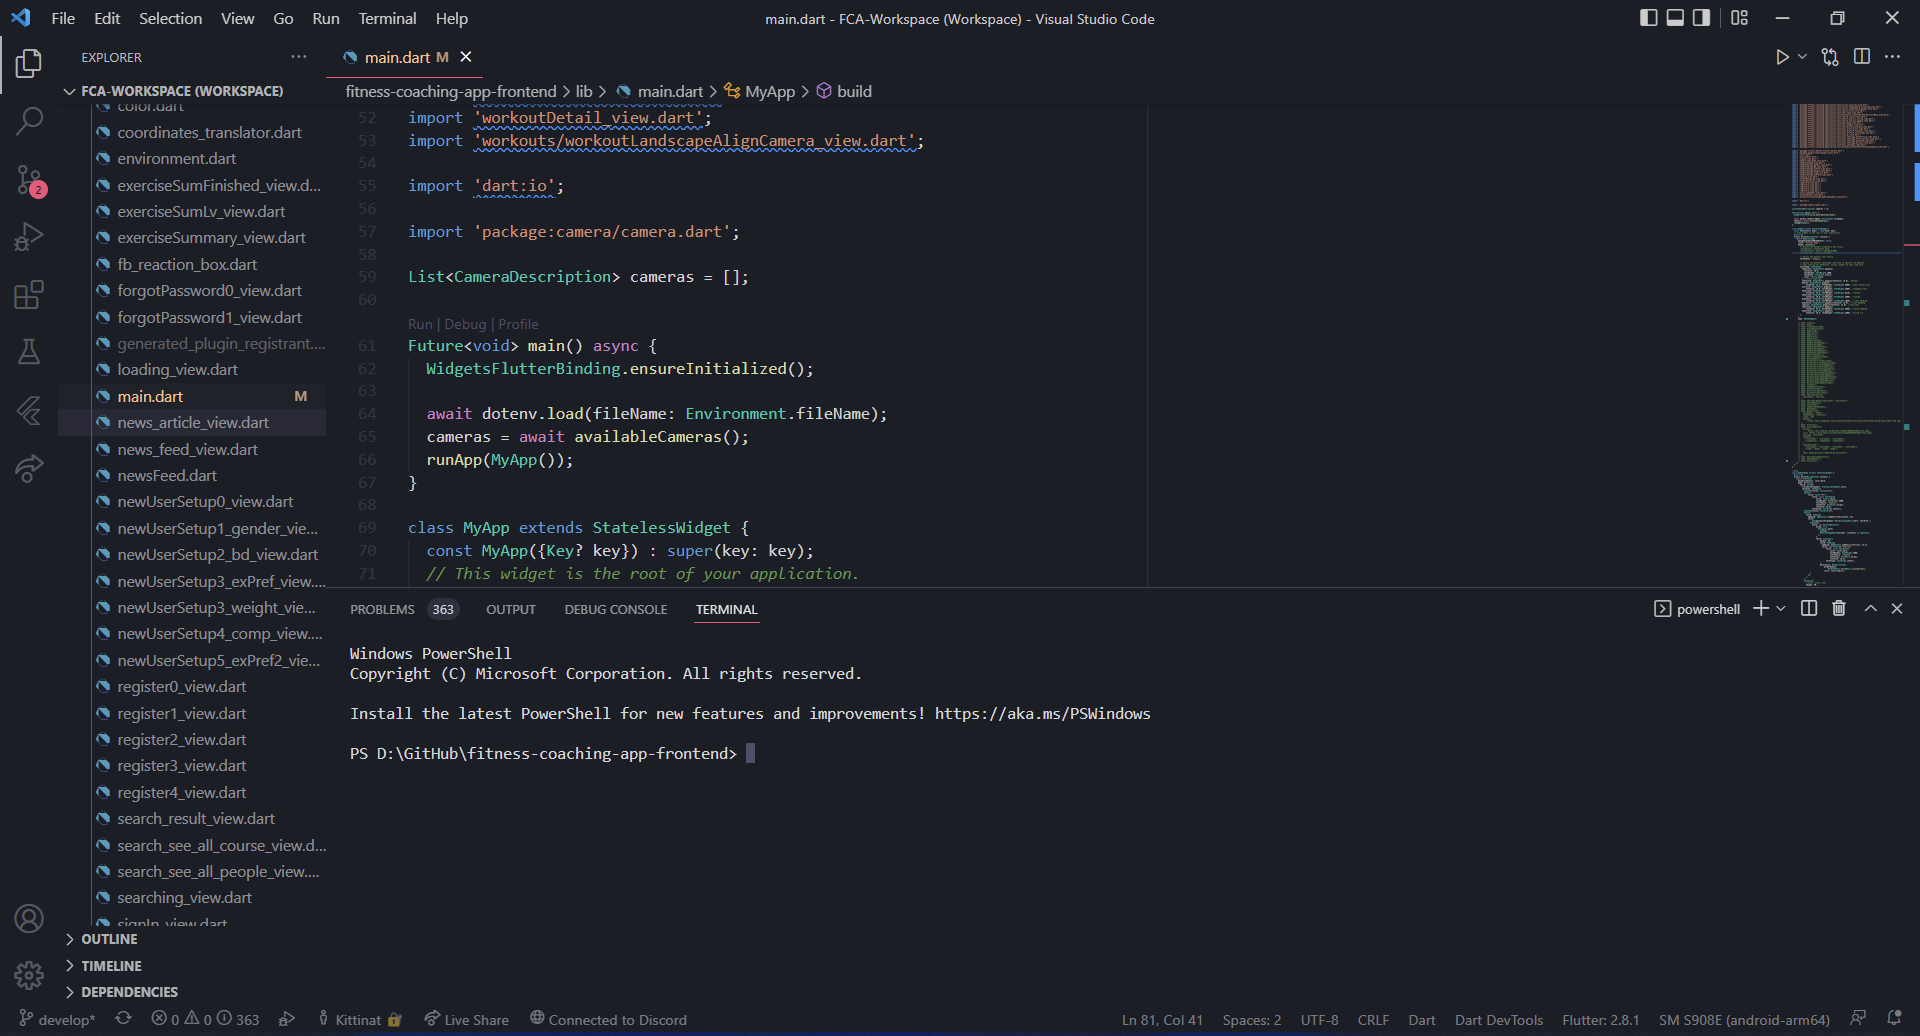
\includegraphics[width=15cm]{./appendix/a-3.png}
        \caption{หน้าต่าง Terminal ที่แสดงขึ้น}
    \end{figure}
    \item ตรวจสอบที่หน้าต่าง Terminal ว่าตำแหน่ง Current Working Directory นั้นได้อยู่ที่ตำแหน่งของ Flutter Project ที่พัฒนาเรียบร้อยแล้ว จากนั้นให้ทำการพิมพ์คำสั่ง flutter build apk เพื่อให้ Flutter ทำการ Build แอปพลิเคชัน
    \begin{figure}
        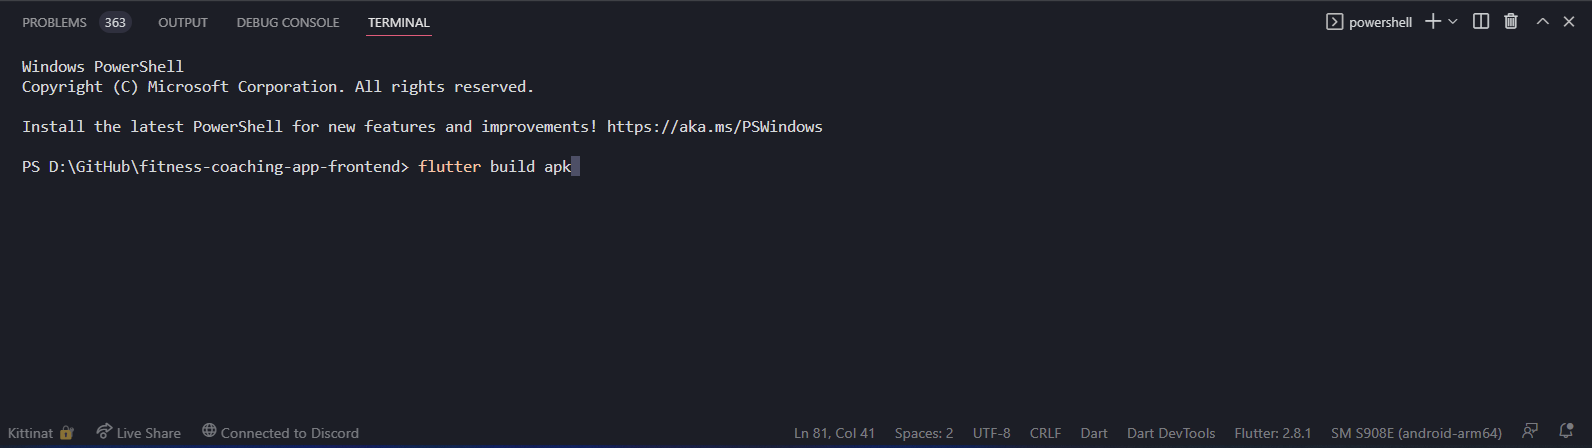
\includegraphics[width=15cm]{./appendix/a-4.png}
        \caption{การพิมพ์คำสั่งเพื่อให้ Flutter ทำการ Build แอปพลิเคชัน}
    \end{figure}
    \item Flutter จะทำการ Build แอปพลิเคชัน ซึ่งจะใช้เวลาชั่วขณะหนึ่ง
    \begin{figure}
        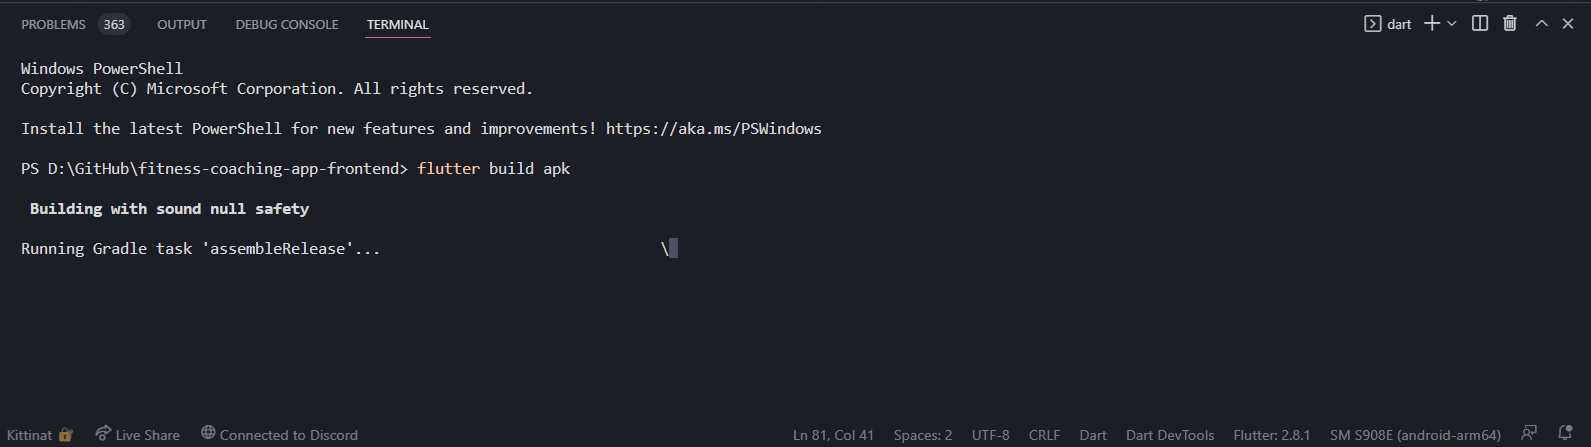
\includegraphics[width=15cm]{./appendix/a-5.png}
        \caption{หน้าต่าง Terminal ซึ่งแสดงการทำงานขณะที่ Flutter ทำการ Build แอปพลิเคชัน}
    \end{figure}
    \item เมื่อ Flutter ทำการ Build แอปพลิเคชันเสร็จเรียบร้อยแล้ว จะมีข้อความแจ้งเตือนที่หน้าต่าง Terminal โดยบอกตำแหน่งของไฟล์ .apk ที่ได้และขนาดของไฟล์ .apk ดังกล่าว คือ <ตำแหน่งโฟลเดอร์ของโปรเจค> \textbackslash build \textbackslash app \textbackslash outputs \textbackslash flutter-apk \textbackslash app-release.apk
    \begin{figure}
        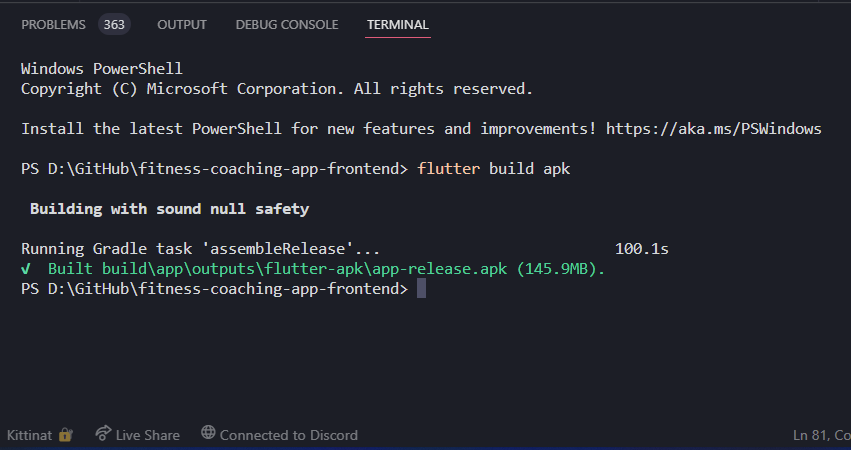
\includegraphics[width=15cm]{./appendix/a-6.png}
        \caption{หน้าต่าง Terminal ซึ่งแจ้งให้ทราบถึงการ Build แอปพลิเคชันเสร็จสิ้น}
    \end{figure}
    \item ไปยังตำแหน่งโฟลเดอร์ที่เก็บไฟล์ app-release.apk ดังกล่าว และนำไฟล์ที่ได้ไปติดตั้งบนสมาร์ตโฟนระบบปฏิบัติการ Android เพื่อใช้งาน
    \begin{figure}
        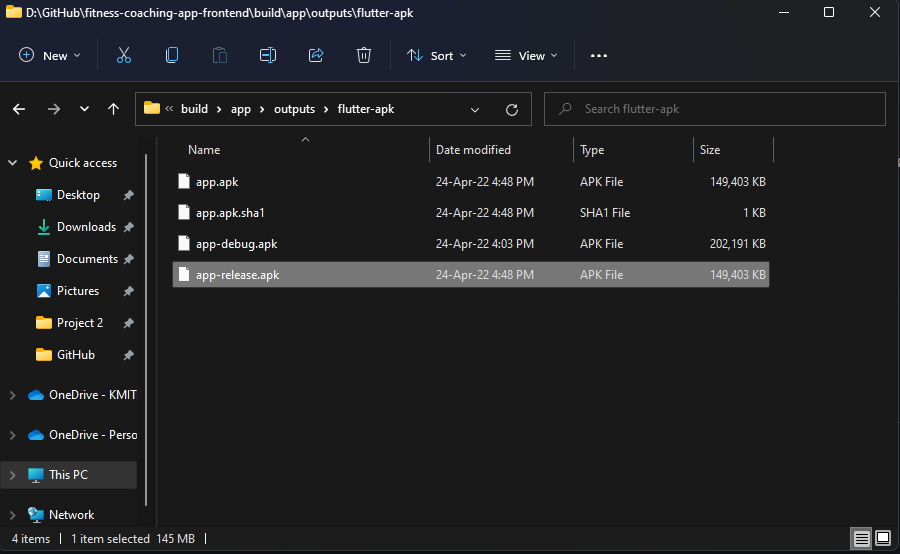
\includegraphics[width=15cm]{./appendix/a-7.png}
        \caption{ตำแหน่งโฟลเดอร์ที่เก็บไฟล์ app-release.apk}
    \end{figure}
\end{enumerate}

\section{การนำแอปพลิเคชันที่ Build เสร็จเรียบร้อยแล้วเผยแพร่ออกสู่สาธารณะผ่าน GitHub}
การนำแอปพลิเคชันที่ Build เสร็จเรียบร้อยแล้วเผยแพร่ออกสู่สาธารณะนั้น ทาง GitHub มีส่วนของการ Release สำหรับการแนบ Source code ของโครงงาน และสามารถแนบไฟล์ .apk เพื่อเผยแพร่สู่สาธารณะได้ โดยมีขั้นตอนดังนี้
\begin{enumerate}
    \item เปิดเว็บไซต์ https://github.com/ และไปยังหน้า Repository ของโครงงาน
    \begin{figure}
        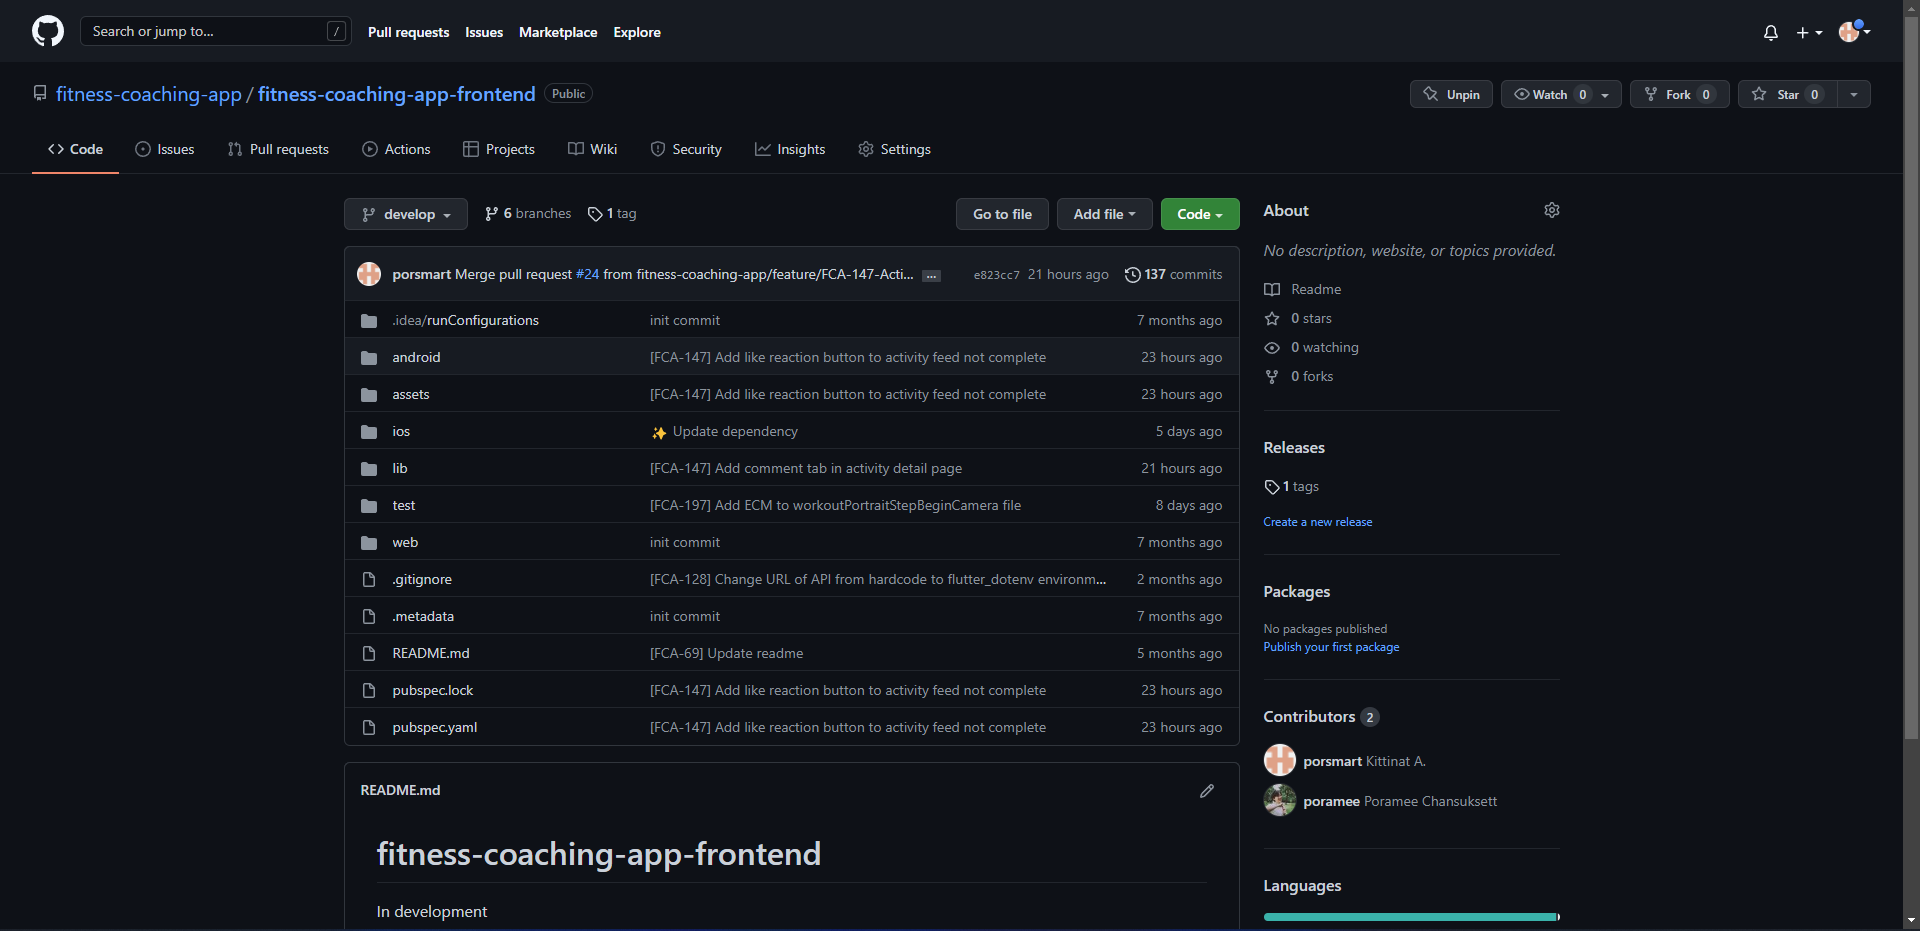
\includegraphics[width=15cm]{./appendix/a-8.png}
        \caption{หน้า Repository ของโครงงานในเว็บไซต์ GitHub}
    \end{figure}
    \item ที่บริเวณด้านขวาของเว็บไซต์จะมีหัวข้อ Release และคลิกเมนู Create a new release เพื่อสร้าง Release ใหม่
    \begin{figure}
        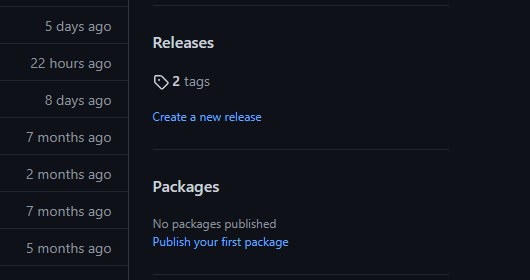
\includegraphics[width=15cm]{./appendix/a-9.png}
        \caption{หัวข้อ Release ในเว็บไซต์ GitHub}
    \end{figure}
    \item จากนั้นหน้าเว็บไซต์จะนำทางไปยังหน้าการสร้าง Release ใหม่ ให้ทำการกำหนดชื่อ Tag ที่จะใช้ (มักจะใช้เป็นชื่อเวอร์ชัน เช่น v1.0.0 เป็นต้น), กำหนด Target ว่าจะใช้ Branch ใดในการแนบ Source code ของการ Release ในครั้งนี้, กำหนดชื่อ Release Title สำหรับหัวข้อ Release และคำอธิบาย
    \begin{figure}
        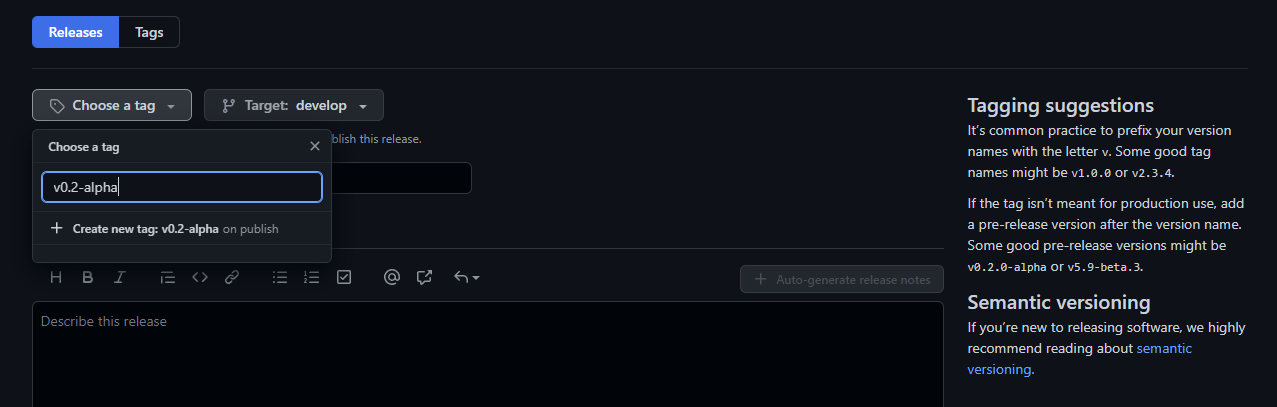
\includegraphics[width=15cm]{./appendix/a-10.png}
        \caption{การกำหนดชื่อ Tag ที่จะใช้}
    \end{figure}
    \begin{figure}
        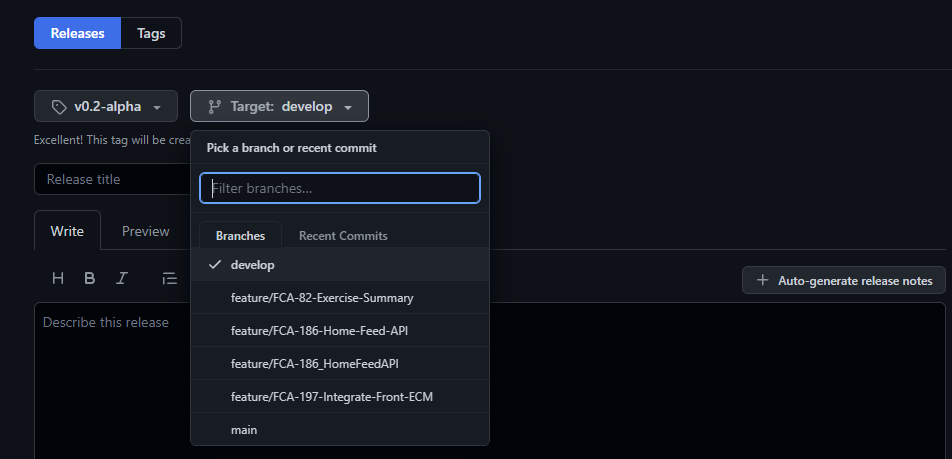
\includegraphics[width=15cm]{./appendix/a-11.png}
        \caption{การกำหนด Target ที่จะใช้}
    \end{figure}
    \begin{figure}
        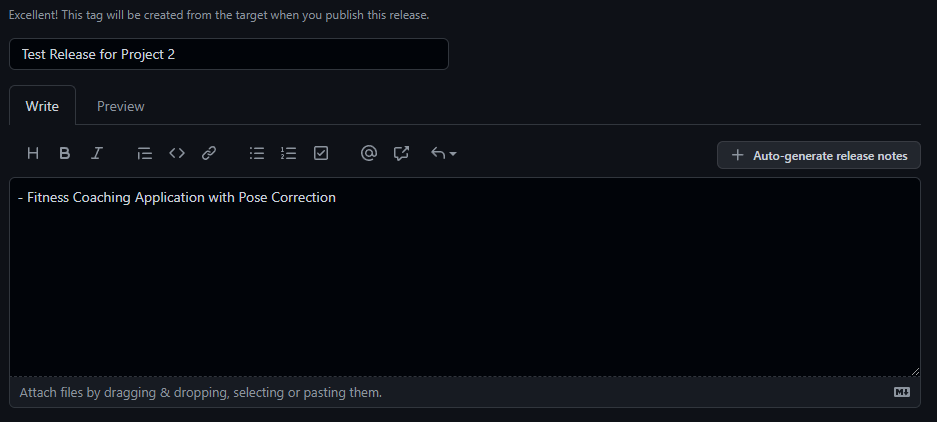
\includegraphics[width=15cm]{./appendix/a-12.png}
        \caption{การกำหนดหัวข้อและคำอธิบายของ Release นี้}
    \end{figure}
    \item เมื่อกำหนดข้อมูลข้างต้นเรียบร้อยแล้วให้ทำการอัพโหลดไฟล์ .apk ที่ต้องการเผยแพร่ใน Release นี้
    \begin{figure}
        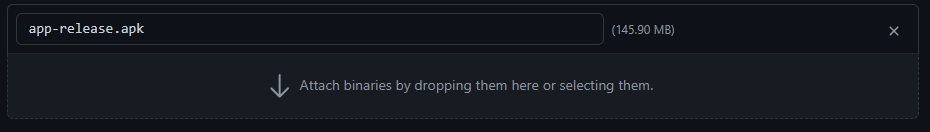
\includegraphics[width=15cm]{./appendix/a-13.png}
        \caption{หน้าต่างการอัพโหลดไฟล์ .apk ที่ต้องการเผยแพร่}
    \end{figure}
    \item หากการ Release นี้ยังไม่พร้อมสำหรับการ Production ให้คลิกที่ปุ่ม This is a pre-release จากนัันคลิกที่ปุ่ม Publish release เพื่อทำการเผยแพร่ Release
    \begin{figure}
        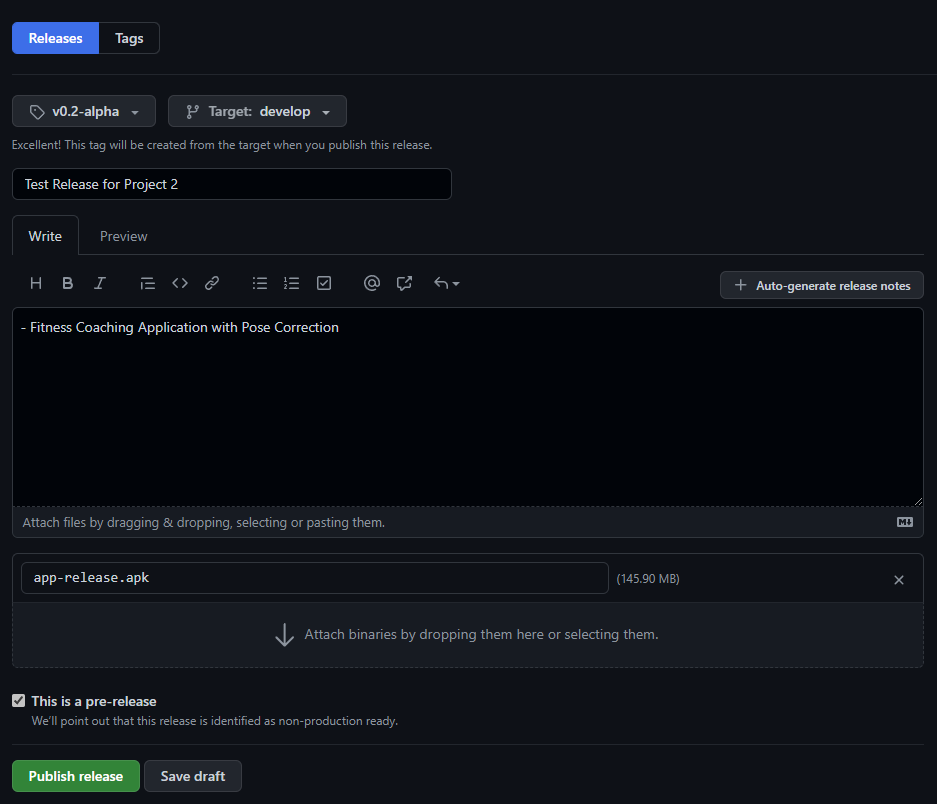
\includegraphics[width=15cm]{./appendix/a-14.png}
        \caption{หน้าต่างการกำหนดข้อมูลต่าง ๆ ของ Release}
    \end{figure}
    \item เมื่อทำการ Release เสร็จเรียบร้อยแล้ว เว็บไซต์จะนำทางไปยังหน้าของการ Release ดังกล่าวที่เผยแพร่สู่สาธารณะเรียบร้อยแล้ว โดยในส่วนของ Assets จะมีไฟล์ไฟล์ .apk และไฟล์ Source code ของโครงงานซึ่งอยู่ในรูปแบบไฟล์ .zip และ .tar.gz
    \begin{figure}
        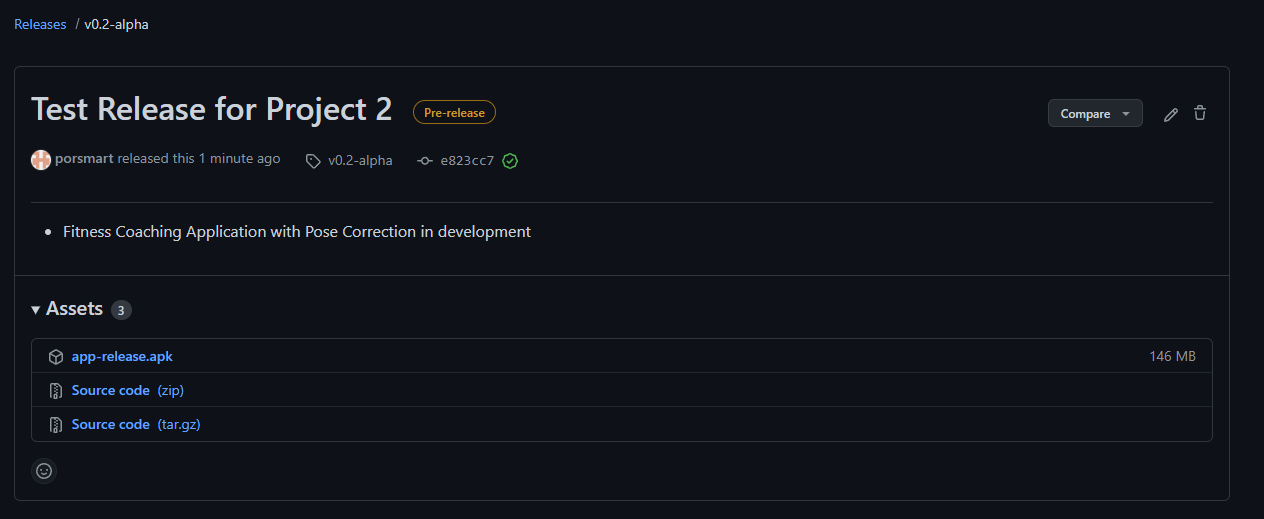
\includegraphics[width=15cm]{./appendix/a-15.png}
        \caption{หน้าต่างการกำหนดข้อมูลต่าง ๆ ของ Release}
    \end{figure}
\end{enumerate}

\section{การ Deploy ระบบ Backend ไปยัง Google Cloud Functions ผ่าน GitHub Actions}
เมื่อได้พัฒนาระบบ API และ Database และได้ Push ไปยัง GitHub Repository เรียบร้อยแล้ว ทาง GitHub มีส่วนของการใช้งาน GitHub Actions สำหรับการ Deploy ระบบ ไปยัง Google Cloud Functions โดยอัตโนมัติ โดยมีขั้นตอนดังนี้
\begin{enumerate}
    \item เปิดเว็บไซต์ https://github.com/ และไปยังหน้า Repository ของระบบ Backend
    \begin{figure}
        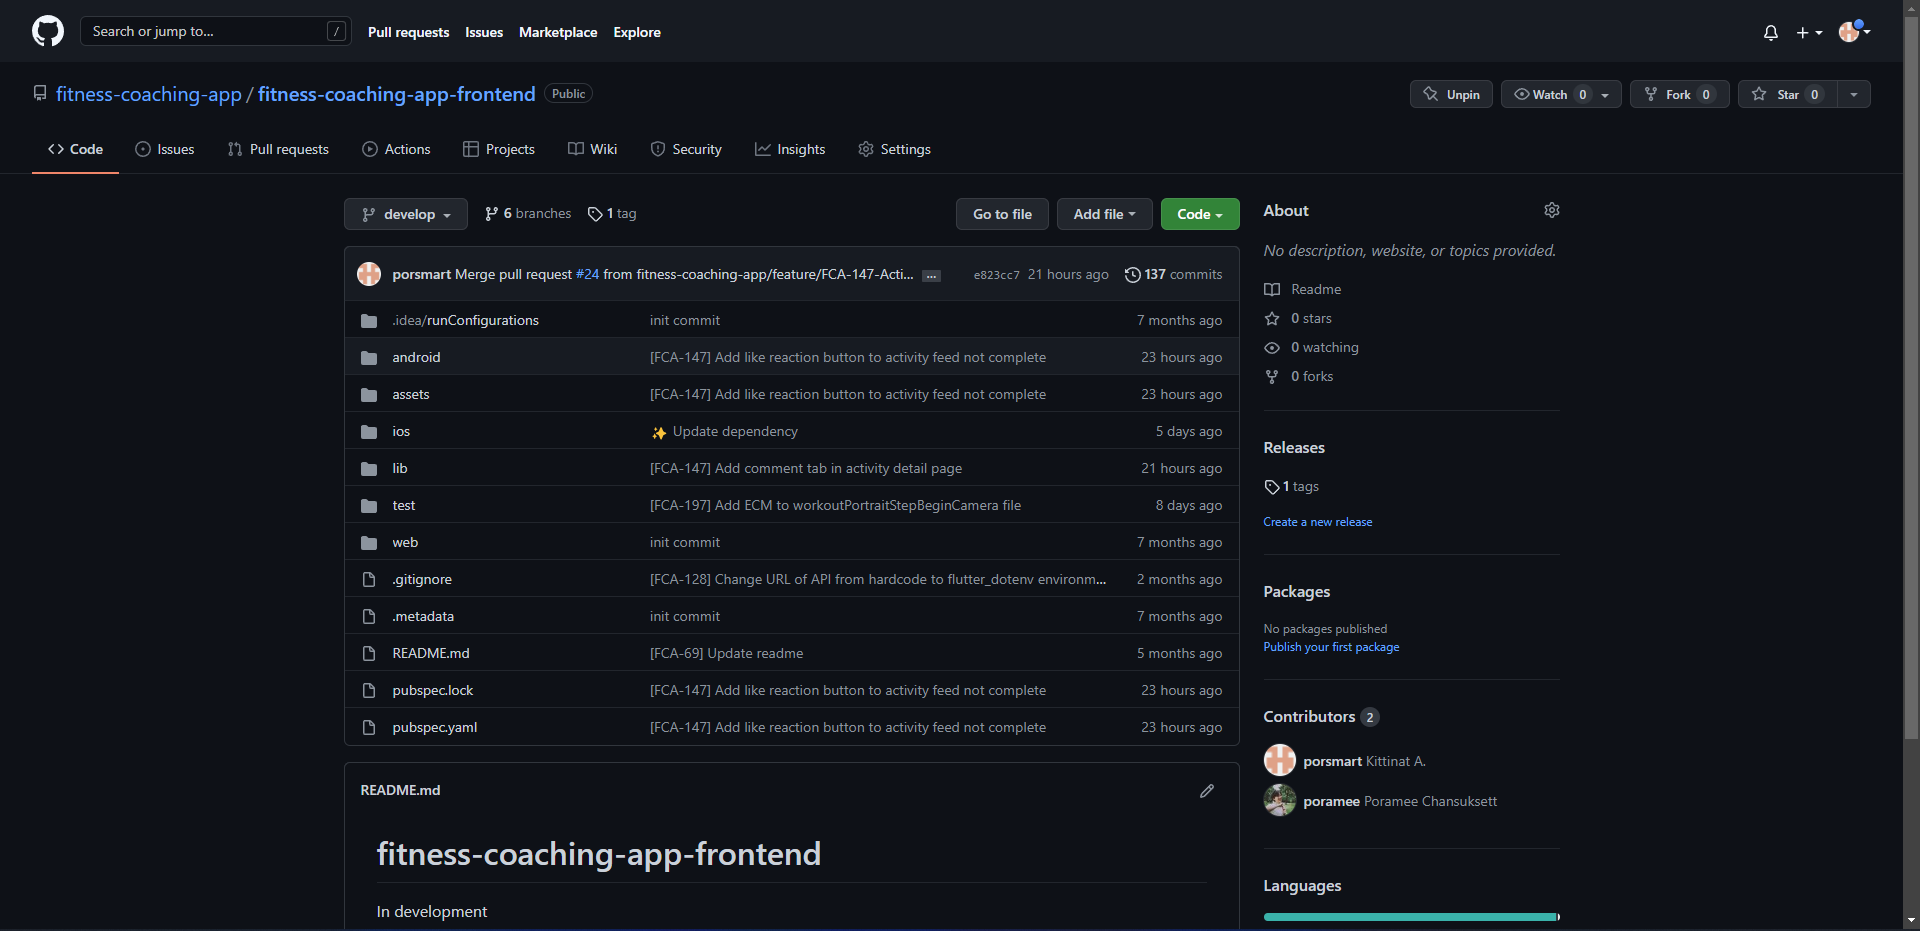
\includegraphics[width=15cm]{./appendix/a-8.png}
        \caption{หน้า Repository ของโครงงานในเว็บไซต์ GitHub}
    \end{figure}
\end{enumerate}